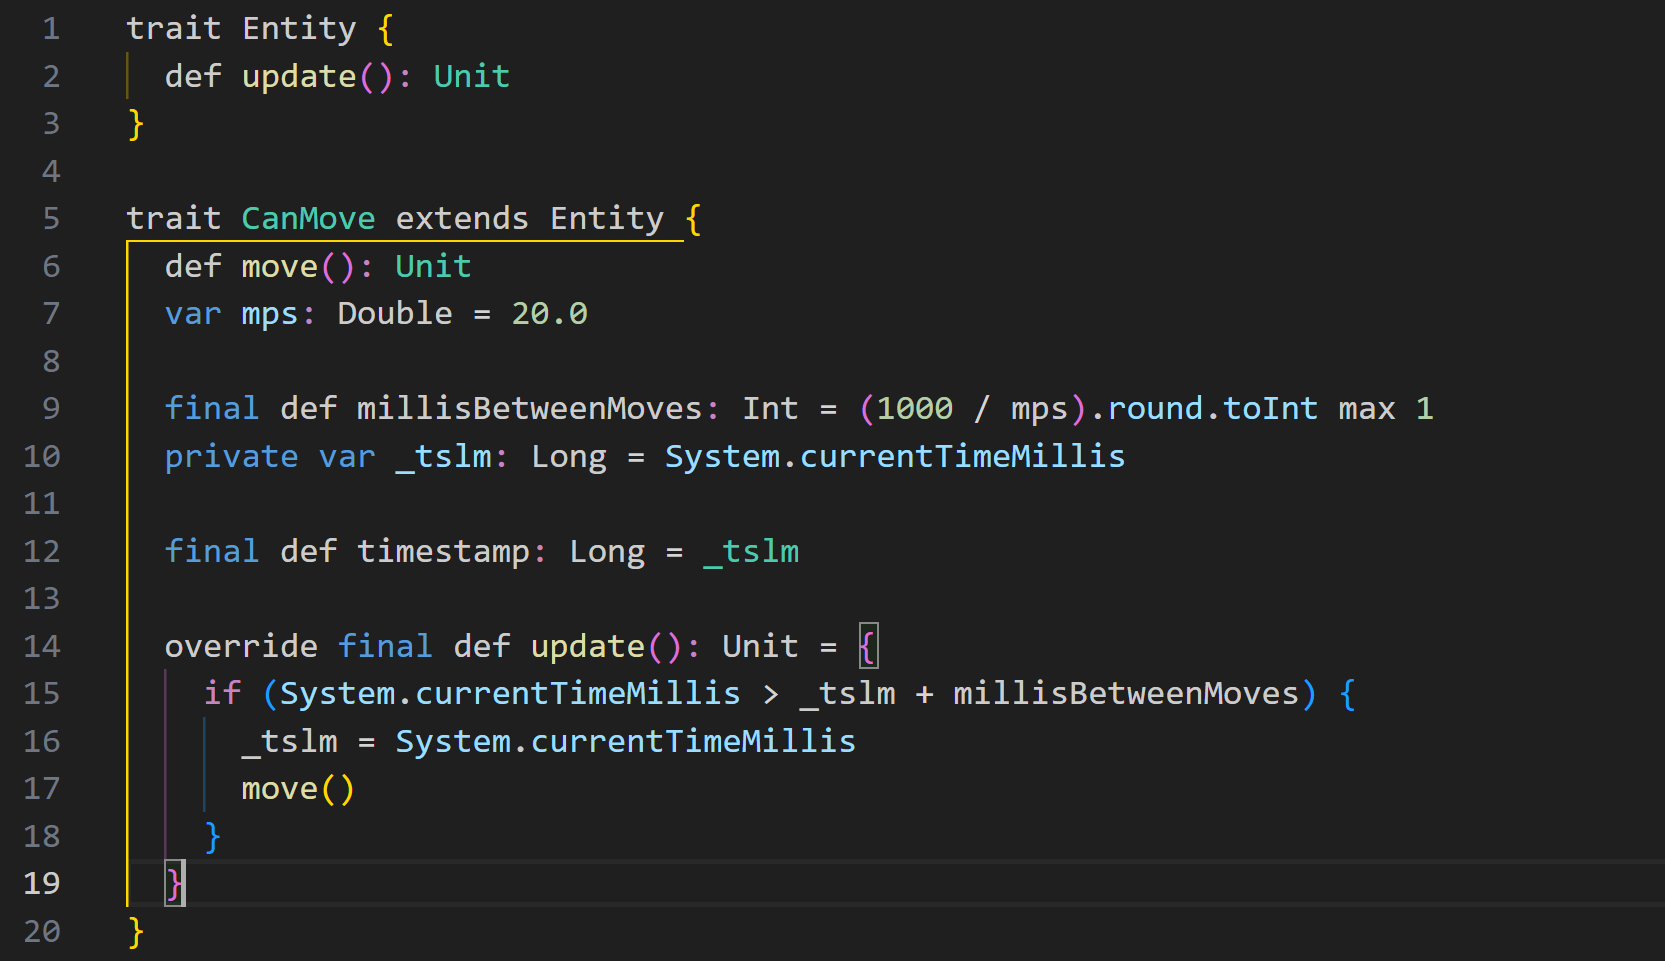
\includegraphics[width=15cm]{fina_koden.png}
I Koden används bara krullparanteser för att markera avslut på kodrader tillhörande prefix.
Detta gör det svårt för oss att bygga upp vilka grupper av kod som tillhör varandra då krullparanteser inte är särskilt starka kännetecken.
Selektiv uppfattning innebär att vi uppfattar det som sticker ut.
Eftersom krullparanteser är ett svagt kännetecken är koden dåligt optimerad för förståelse.
Det finns heller inga visuella kännetecken som t.ex färg. Vilket också gör det svårt att få en förståelse.

Koden brister i kontext i både variabelnamn och funktion.
Detta gör att vi har svårt att komma ihåg vad som står skrivit då vi inte vet vad koden ska användas till.
Kunskap i världen(norman) vissa variabelnamnen, som t.ex _tslm, gör det svårt att förstå kontexten.




